\documentclass[a4paper]{article}

%% Language and font encodings
\usepackage[english]{babel}
\usepackage[utf8x]{inputenc}
\usepackage[T1]{fontenc}

%% Sets page size and margins
\usepackage[a4paper,top=3cm,bottom=2cm,left=3cm,right=3cm,marginparwidth=1.75cm]{geometry}

%% Useful packages
\usepackage{amsmath}
\usepackage{graphicx}
\usepackage[colorinlistoftodos]{todonotes}
\usepackage[colorlinks=true, allcolors=blue]{hyperref}

\title{Modelo de sistema  de apoyo al diagnóstico de melanoma utilizando redes convolucionales}
\author{Pablo Fernando Guzman Quispe}

\begin{document}
\maketitle
%%%%%%%%%%%%%%%%%%%%%%%%
%\begin{abstract}
%Your abstract.
%\end{abstract}
%%%%%%%%%%%%%%%%%%%%%%%%
\section{Descripción de la Realidad del Problema}

El melanoma es el tipo de cáncer de piel más mortífera [1]. A pesar de esto sólo representa el 4\% de todos los cánceres de piel, que causa el 75\% de todos los casos de muerte [7][3]. Pero también es una de la más fáciles de curar, solo si es detectado en etapas muy tempranas. Sin embargo, si es detectado muy tarde lo más probable es que haya penetrado a dentro de la piel con riesgo de metástasis [5]. 

La presencia de melanocitos en cualquier parte del cuerpo causa el melanoma. La intensa exposición de la piel a la radiación ultravioleta es una de las principales causas [7]. El cual por una rápida multiplicación celular forma un tumor maligno [5]. 

Entre los métodos para detectar y dar diagnostico tenemos a la Biopsia, el cual da un diagnóstico definitivo. Pero el procedimiento puede causar metástasis por lo que se permite solo cuando se va intervenir quirúrgicamente dentro de un mes. También ocasionando molestias al paciente por ser operaciones invasivas [7].  En estos días. Los métodos para la detección de melanomas malignos utilizan imágenes dermatoscópicas.  Pero este método depende mucho de la experiencia del médico, lo que lo hace con una exactitud de 75-84\% [7]. Siendo un método no invasivo, pero sin la exactitud de una biopsia.

Apostando por los métodos no invasivos y utilizando las imágenes dermatoscópicas. Una forma de aumentar la exactitud del diagnóstico es utilizando asistencia de computador. Esto no indica que el computador diagnosticara, su única labor será la extracción de características que el ojo humano puede no percibir, como variación de color, asimetría, características de textura, bordes sin definir [7]. Ayudando al rápido diagnóstico del médico.

Existen muchos algoritmos ya implementado en los sistemas de extracción de información y reconocimiento de melanomas tales como seven-point checklist, ABCD rule y the Menzies method los cuales dan una mayor exactitud para el diagnóstico de cáncer de piel [2][3][4]. 

Para cada método es necesario el uso indispensable de las imágenes dermatoscópicas, también para aclarar que los métodos solo sirven para identificar y extraer características. Por ende, las imágenes necesitan ser pre-procesadas antes de aplicar los métodos. Proporcionando los resultados de la extracción de características, los cuales pueden ser procesadas por una inteligencia artificial para la clasificación e identificación de cáncer de piel [4]. Esto quiere decir que no solo depende del método que se va aplicar a las imágenes, sino que también depende mucho del tipo de inteligencia artificial que se va usar o del pre-procesamiento previo antes de la extracción de características.


\section{Estado del arte}

\subsection{Requerimientos para detección de melanoma}

Para la detección de melanomas. Debemos entender cuál es su origen, el cáncer a la piel comienza como una lesión plana en la superficie de la piel. Por ende, este aparenta ser un lunar común, pero después de cierta condiciones y estadíos. Su tamaño comienza incrementar anormalmente y se termina convirtiendo en un tumor maligno [1]. A esta anomalía en la piel se le considera como cáncer a la piel o melanoma.
El cáncer a la piel causa la muerte si no es tratado apropiadamente, cuando el cáncer de piel se profundiza hasta sobrepasar las capas de la piel, las opciones de sobrevivir son muy escasas [1]. Por eso existen muchas técnicas de detección.
Las técnicas detección que usan por ser un método no invasivo son mediante la visión o llendo al ámbito de las computadoras la visión computacional. 


%\begin{figure}
%\centering
%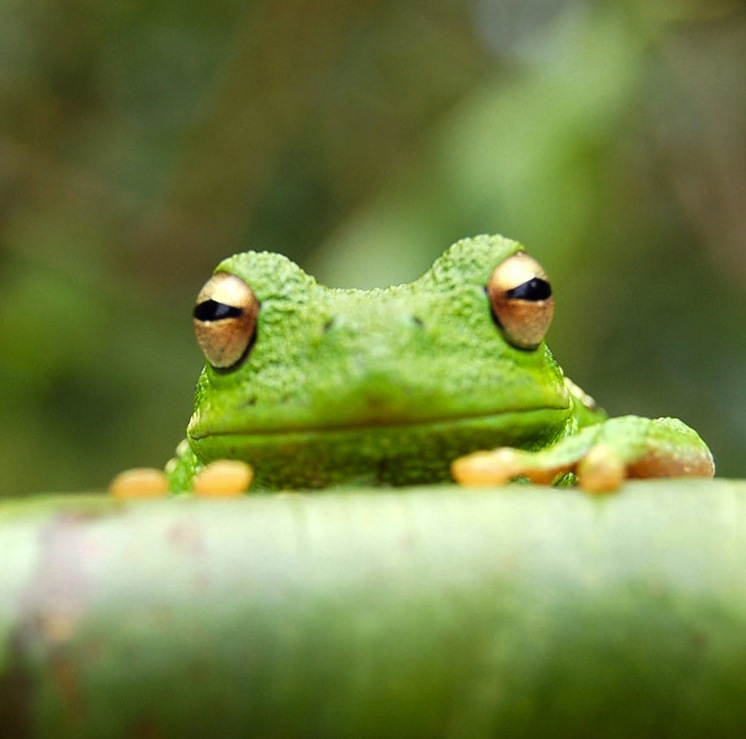
\includegraphics[width=0.3\textwidth]{frog.jpg}
%\caption{\label{fig:frog}This frog was uploaded via the project menu.}
%\end{figure}

\subsection{Detección de melanoma computarizado}

La detección de melanoma mediante la visión computacional se ha vuelvo una gran ayuda para el diagnóstico. Teniendo en cuenta que la precisión de diagnóstico mediante la experiencia y vista humana es de un 75\% al 84\%. Por otro lado, la visión computación con inteligencia artificial  está teniendo buenos resultado de precisión [3], siendo más rápido y eficaz. Esto no quiere decir que la visión computación es mejor que la inteligencia humana, sino que puede extraer características que son casi imperceptibles o que son ignoradas por el ojo humano.
Para realizar el diagnóstico existen varios métodos como las invasiva (biopsias y análisis citológicos) y las no invasivas(mediante la observaciones de patrones característicos del melanoma) [3]. Los sistema computacionales para el diagnóstico usan métodos no invasiva que sólo necesitan de una fotografía en alta definición del lunar sospechoso para melanoma para su detección.

Imagenes dermatoscópicos\\
La dermatoscopia es una técnica de examinación no invasivo basada en la luz incidente y otro factores que permite la posibilidad de examinar visualmente las superficie de la piel. Por esa razón la examinación por este método es mejor que solo por el ojo humano [6].
Las imágenes dermatoscópicos son la foto tomadas por el procedimiento de la dermatoscopia lo cual en formato digital será procesado por el sistema computacional.
Para obtener las imágenes dermatoscopios muchos trabajos han adquiridos DataSet que provienen de distintas universidades o clínicas. Por ejemplos, para melanomas, el hospital de  Keio University tiene 30 imágenes, la universidad de Naples and Graz tiene 75 imágenes [7] y  el hospital de Vienna con 26 imágenes[4].

Sistema computacional\\
El sistema computacional como primer paso usa imágenes digitales, el cual puede aplicar múltiples métodos para la extracción de características. Los cuales son parte de la metodología, cabe resaltar que seguna la extracción de características define también la precisión del el sistema computacional. es por eso que los métodos más usados como las reglas ABCD donde A es simétrica, B es bordes, C es color y D es diámetro, son unos de los más usados en la gran mayoría de sistemas computacionales [2][3][5]. 


\subsection{Métodos aplicados}

Los métodos son las formas de cómo se extraerán las características de los lunares o melanomas, la gran mayoría de ellos se van en su forma como: a) perímetros b) color c) textura d) luminiscencia [3].
Los métodos más aplicados para la extracción de características de las imágenes dermatoscópicas en los sistemas computacionales según las investigación son los siguientes: 1) reglas de ABCD ; 2) Análisis de patrones;3) Métodos Menzies; 4) seven-point checklist; y 5) Análisis de textura [4].

Reglas de ABCD:\\ 
En este método investiga en la imagen la características del lunar como es: la asimetría donde la lesión es dividida por las abscisas para el análisis, los bordes es  donde se define es la forma de la lesión, el color es examinada dentro de la lesión determinando la cantidad de colores presentes, y los números estructuras diferenciadas como los pigmentos, glóbulos, cicatrices o cualquier forma de ruido [4].
Se resalta que hay un método también ABCD que utiliza el diámetro como elemento para el análisis y que lo representa como D. 
Estructuras diferenciadas:\\
Es un método que ha sido agregado en las muchos métodos como la regla ABCD y es usado por hallar irregularidades, falta de homogeneidad al examinar la superficies de la lesión. También es usado en los métodos como Menzies y  Seven-point checklist [4].
Análisis de patrones:\\
Este método de análisis se centra especialmente en la identificación de  patrones los cuales sean dividido en globales como (ronchas, glóbulos y multicomponente no especificados) y locales como (red de pigmentos, pecas lunares, cicatrices y hiper o hipo pigmentación de la piel) [4].
Métodos Menzies:\\
Este método no trabaja igual que todos, ayq ue se encarga de observar la características negativas como que el lunar sea simétrico, que el color sea homogéneo dentro de la lesión, bordes bien definidos. En resumen lo que trata de hacer es que demostrar que no es un lunar maligno o melanoma. Si no consigue demostrarlo indica que lo es [4].
Seven-point checklist:\\
En este método se trabaja con 7 criterios que se basan en la características cromáticas y las formas y/o las texturas de la lesión. estos criterios son: a) Atipica pigmentación; b) Veloz azul-blanquecinos; c) Atípico patrones vasculares; d) Estrías irregulares; e) Puntos irregulares; f) Manchas irregulares; g) Estructuras de regresión [4].
Cada unos son considerados para la identificación pero con diferente pesos en el diagnóstico, por lo tanto las imágenes digitales pasa por estos procesos según el orden en que se van presentado la evidencias. 
Análisis de textura:\\
En este método consiste en intentar cuantificar la percepción de la textura de la lesión. usando las siguiente etiqueta como a) Fino; b) Rugoso; c) Irregular. Para identificar, medir y comparar la diferencia entre ellos usan 2 tipos de categorías como la estadística que lo define mediante análisis de escala de grises y la estructural que define según lo establecido [4].

Cada uno de los métodos son usados según la necesidad de cómo identificar los melanomas. cabe resaltar que los más usados entre estos métodos en los sistemas computacionales son la regla ABCD y estructura diferencias. la razón de que el método estructuras diferencias sea de la más usadas es que puede tomar parte de otros métodos.


%\begin{table}
%\centering
%\begin{tabular}{l|r}
%Item & Quantity \\\hline
%Widgets & 42 \\
%Gadgets & 13
%\end{tabular}
%\caption{\label{tab:widgets}An example table.}
%\end{table}

\subsection{Diagrama de flujo}

Los diagrama de flujo son la representación de cómo las imágenes digitales (dermatoscópicas) pasarán por el sistema computacional para la identificación y/o clasificación del melanoma. Tener en cuenta que el diagrama de flujo puede variar según el investigador pero la gran mayoría tiene los procesos fáciles de identificar. 
los procesos más generales obtenidos son los siguiente:
Adquisición de imágenes:\\ 
En este proceso se indica que las imagen será obtenida y tendra que es la entrada de sistema computacional. especificado como parte del flujo por la mayoría de los artículos de investigación y por ende tiene su relevancia en este flujo de proceso.
Puede ser también identificado con el nombre de input imagen  o Imagen acquisition y en otros casos como input imagen skin lesion [8].
Segmentación de la imagen:\\ 
Este proceso es el segundo en la mayoría de las investigación el cual es un paso esencial en el flujo. en este proceso en donde se llega ha hacer el procesamiento de la imagen y dejarlo listo para la extracción de características. 
Pero antes de realizado el análisis para por un proceso en el cual consiste en eliminar el ruido de la imagen antes del procesado de la imagen. En algunos artículos puede identificarse que lo dividen en dos procesos como Preprocesamiento y segmentación [2][4][5]. .
El proceso más conocido como preprocesamiento de la imagen es el DULL RAZOR el cual se encarga de eliminar el ruido de las vellosidades mediante un algoritmo[8].
Los procesos que se llevan son la obtención  de escala de grises, obtención de bordes y captura de superficie, el cual será usado para la extracción.
Puede ser también identificado en otros artículos como Pre-procesamiento o procesamiento de imagen porque puede no se encuentre el proceso de segmentación [9].
Extracción de características:\\
Este proceso suele ser el tercero o cuarto, siempre despues despues de procesamiento de imágenes y tiene como tarea principal identificar las características según los métodos especificados.
La salida de este proceso es muy importante para el siguiente proceso, ya que no se tratara la imagen sino los datos extraídos de las imágenes procesadas.
Su nombre no varía mucho en los demás artículos por ser un proceso clave en la investigación y detección de melanomas.
Clasificador
Este proceso  clave del flujo su importancia recae en que es una inteligencia artificial y que permitirá clasificar o identificar si es o no un melanoma. la cual puede haber sido implementada de múltiples maneras pero según el método de inteligencia artificial depende  mucho también la precisión del diagnóstico. Con un buen método y bueno casos de pruebas buenos resultados obtendrá el sistema computacional [9].
El clasificador por ser una inteligencia artificial tiene dos subprocesos los cuales son uno de entrenamiento o fase de aprendizaje, la fase de testeo para corroborar que el diagnóstico es correcto [8].
Después de esos dos procesos ya estará disponible para dar diagnostico con un nivel precision mas certero. siempre recordar que nunca se obtendrá la precisión del 100% .


\subsection{La precisión de los métodos de detección}

La precisión de los sistemas computacionales son  muy variantes por los métodos a usar y las inteligencia artificial que se implementó. También tiene mucho que ver el DataSet porque según la calidad de la imagen digital.
Según el artículos de Aswin. R. B., J. Abdul Jaleel y Sibi Salim usando la técnica de ABCD entendiéndose como asimetría, bordes, colores y diámetro, teniendo como dataset entre como imágenes digitales de  cancerosa y no cancerosas un total de 50. llegando a un resultado como mayor precisión al 88\%. Entrando como un detector de cancer efectivo [1].
Segun el articulo de IliasMaglogiannis y Charalampos N. Doukas nos da una tabla clasificadora que según el algoritmo que se usa en el clasificador puede dar un valor variado en la precisión del diagnóstico. utilizando redes neuronales para el clasificador nos una una precisión de 85 al 89\% lo cual entra entre los parámetro aceptable para un identificador. Usando métodos estadísticos en el clasificador la mejor marca adquirida es de un 89\% y raras veces bajando al 71\%. Usan el clasificando basados en reglas, la precisión varía entre 83.2\% y 86.3\% por diagnóstico. Así continúa dando más datos para su análisis [4].
Según el artículo de Rebecca Moussa, Firas Gerges, Christian Salem, Romario Akiki, Omar Falou, y Danielle Azar[3], usando los metodos de extraccion de caracteristicas ABCD y el como clasificador k-Nearest Neighbors. obtiene un precisión de 89\% según su DataSet. teniendo en cuenta que solo uso el 40\% de ella.
Según el artículo de Kouhei Shimizu, Hitoshi Iyatomi, M. Emre Celebi, Kerri-Ann Norton, y Masaru Tanaka [7]. El cual implementa cuatro clasificadores para detectar cuatro tipos de cáncer de piel  como el melanoma, nevos, carcinoma de células basales y Queratosis seborreica. usando métodos de extracción como los colores , texturas y regiones afectadas. obteniendo un índice de precisión de 90\% al diagnóstico de cualquiera de las cuatra tipos de cáncer.
Según en el artículo Arushi Bhardwaj y Dr. J.S Bhatia [2], usando inteligencia artificial que proporciona Matlab 2013a y los métodos de extracción de características ABCD obtuvo buenos índices de precisión para una detección temprana de melanoma.
Según el artículo de Anna N. Yaroslavsky, Cecil Joseph, Rakesh Patel, Bo Fan, Alona Musikansky, Victor A. Neel y Robert Giles [10]. usando método muy distinto que usa polarización óptica y Imágenes pulsadas terahertz, obtiene una precisión de 95\% al 98\% para el diagnóstico de melanoma.
habiendo observado todos lo casos en que ha usado los métodos, inteligencias artificiales y procesamiento de imágenes. se obtiene muy buenos resultados con las imágenes dermatoscopios y con el método de extracción de características ABCD .Pero para nuestro proyecto usaremos un método distinto de inteligencia artificial llamado DeepLearning. en cual es una técnica nueva en este ámbito. Por su forma casi distinta de procesar la imagen y clasificarla.

\section{Objetivos del Problema}
\subsection{Objetivo General}

Proponer un sistema de apoyo al diagnostico de melanomas utilizando como clasificador los algoritmos de aprendizaje automático llamado Deep Learning.
\subsection{Objetivos Específicos}
\begin{enumerate}
\item Investigar estado del arte del tema.
\item Investigar melanoma y sus diagnósticos
\item Investigar sobre deeplearning y el diagnóstico
\item Proponer los elementos constitutivos del modelo
\item Evaluar y validar el modelo
\item Redactar la investigación.

\end{enumerate}

\bibliographystyle{alpha}
\bibliography{sample}

\end{document}